% SyncTrace — Manuscript for Multimedia Tools and Applications (Springer)
% Template: sn-jnl.cls (Springer Nature official, v2.1)
% Submit as a single .tex document with attached figures; compile with pdflatex.

\documentclass[sn-basic,Numbered,referee]{sn-jnl}

\usepackage{graphicx}
\usepackage{multirow}
\usepackage{amsmath,amssymb,amsfonts}
\usepackage{amsthm}
\usepackage{mathrsfs}
\usepackage[title]{appendix}
\usepackage{xcolor}
\usepackage{textcomp}
\usepackage{booktabs}
\usepackage{url}
\usepackage{array}
\usepackage{algorithm}
\usepackage{algpseudocode}
\usepackage{float}


\makeatletter
\let\savedSetFootnoteHook\SetFootnoteHook
\makeatother

\newtheorem{theorem}{Theorem}[section]
\newtheorem{proposition}[theorem]{Proposition}
\newtheorem{lemma}[theorem]{Lemma}

\raggedbottom

\begin{document}

\title[SyncTrace]{SyncTrace: real-time audio--video deepfake detection via self-supervised contrastive misalignment learning and localizable spatiotemporal attribution}

\author*[1]{\fnm{B.} \sur{Vizzotto}}\email{user@example.com}
%\author[2]{\fnm{B.} \sur{Second}}\email{second@example.com}

\affil*[1]{\orgdiv{Independent Research}, \orgname{SyncTrace Project}, \orgaddress{\city{}, \country{Brazil}}}
%\affil[2]{\orgdiv{}, \orgname{}, \orgaddress{\city{}, \country{}}}

\abstract{%
Audio--video deepfakes, commonly known as \emph{lip-sync forgeries}, have become one of the most socially damaging classes of generative-media manipulation, yet their detection remains fragile: state-of-the-art detectors are trained on large corpora of synthetically forged media, generalize poorly across manipulation pipelines, and offer little forensic insight beyond a binary verdict. We propose \textbf{SyncTrace}, a multimodal forensic framework that reformulates audio--video deepfake detection as a problem of \emph{self-supervised contrastive misalignment learning}: the model is trained exclusively on authentic video clips and learns the distribution of legitimate lip--speech synchronization, so that spatial, temporal, and spectral deviations from this learned manifold produce an anomaly signal with automatic localization. Three contributions depart from the current literature. First, we introduce a \emph{pseudo-forgery generator with continuously controllable severity} built on a facial-landmark backend, which injects calibrated visual and audio degradations into authentic media and emits pixel-level and frame-level ground truth without any human annotation; training requires no real deepfake corpus. Second, we design a hybrid \emph{Mamba--Attention encoder} (\texttt{SyncEncoder}) that fuses mel-spectrogram and depthwise-CNN video features with a sparse frame-selection mechanism driven by mouth activity, attaining competitive discriminative capacity at a fraction of the compute of full transformer backbones. Third, we attach a \emph{Spatiotemporal Attribution Engine (SAE)} that converts the anomaly embedding into per-frame GradCAM heatmaps, canonical facial-region attributions, and spectro-temporal audio band scores, evaluated against ground truth with objective localization metrics (mean intersection-over-union, Precision@k, and frame-level AUROC). In addition to a binary verdict, the system regresses a continuous \emph{manipulation severity} score in $[0,1]$, a capability absent from prior detectors. We implement the full pipeline with reproducible CI/CD automation and validate equivalence between the PyTorch reference and a quantized INT8 ONNX graph, which runs a complete analysis pass in roughly 15~ms on a commodity CPU, making the framework suitable for edge and real-time deployment. Experimental protocols, benchmark harnesses, and reference implementations are released publicly to support reproducibility.}

\keywords{deepfake detection, audio--video forensics, contrastive learning, self-supervision, explainable AI, state-space models, Mamba, lip-sync forgery, ONNX quantization}

\maketitle

\section{Introduction}
\label{sec:intro}

The rapid maturation of generative models has dramatically lowered the cost of producing convincing synthetic media. Among the resulting threats, audio--video lip-sync forgeries stand out for their deceptive simplicity: only the mouth region and the accompanying speech track need to be re-synthesized, leaving the remainder of the video untouched, which defeats detectors that reason over global image statistics. The consequences for authentication-critical contexts---journalism, legal evidence, political communication, and identity verification---have motivated an intense research effort on computational forensics, surveyed broadly under the umbrella of deepfake detection.

Existing detection systems share a common vulnerability: they are trained discriminatively on large collections of \emph{known} forgeries and therefore inherit the distribution of the synthesis pipelines that generated those forgeries. When confronted with a manipulation produced by a different generator, a different resolution regime, or a post-processing chain, detection performance degrades sharply. This cross-manipulation fragility is well documented and remains arguably the central open problem in the field. A second, less explored deficiency concerns \emph{transparency}: current systems reduce a forensic question to a scalar probability, whereas investigators and downstream systems increasingly require an answer to \textit{where} and \textit{how much} a video has been manipulated---which frames, which facial region, and which spectral band carry the evidence of forgery.

In this paper we address both deficiencies with \textbf{SyncTrace}, a multimodal forensic framework built around a single conceptual pivot: instead of learning to recognize forged media, SyncTrace learns to model \emph{legitimate} audio--video synchronization and detects forgeries as \emph{anomalous deviations} from that model. The key technical enabler is a pseudo-forgery generator that, given an authentic clip, injects spatial, temporal, and spectral degradations at a \emph{continuously controllable} severity level and simultaneously emits automatic ground-truth masks over frames, pixels, and frequency bands. The generator makes it possible to train a \emph{contrastive misalignment learner} exclusively on authentic media, with the synthetic degradations acting as negative anchors whose severity label supervises both the contrastive margin and a severity regression head. At inference time, any input whose embedding deviates from the authentic manifold receives an anomaly score; because the training signal is dense and multi-granular, this anomaly can be \emph{localized} back to frames, facial regions, and mel-frequency bands through gradient-based attribution.

The four scientific contributions of this work are as follows:
\begin{itemize}
  \item \textbf{A self-supervised contrastive formulation of audio--video deepfake detection} trained only on authentic media, with automatically generated pseudo-forgeries of controllable severity. This eliminates dependence on corpora of labeled synthetic forgeries and, for the first time in the literature we are aware of, supports continuous \emph{severity regression} of manipulation intensity.
  \item \textbf{A hybrid Mamba--Attention backbone} (\texttt{SyncEncoder}) with sparse frame attention driven by mouth activity, providing strong discriminative capacity at low computational cost, with a full analysis of the accuracy--efficiency trade-off (FLOPs, latency, parameters).
  \item \textbf{Localizable explainability}, through a Spatiotemporal Attribution Engine that maps the anomaly embedding to per-frame heatmaps, canonical facial-region attributions, and spectro-temporal audio band scores, evaluated with objective localization metrics (mean IoU, Precision@k, AUROC) rather than qualitative inspection.
  \item \textbf{Edge-deployable inference with verifiable equivalence}: an ONNX export pipeline with INT8 dynamic quantization whose outputs match the PyTorch reference to machine precision, enabling real-time analysis ($\sim$15~ms per clip on a commodity CPU) suitable for on-device and streaming forensics.
\end{itemize}

The remainder of the paper is organized as follows. Section~\ref{sec:related} positions SyncTrace against recent audio--video forgery detection and self-supervised approaches. Section~\ref{sec:method} describes the pseudo-forgery generator, the contrastive learner, the backbone, and the attribution engine. Section~\ref{sec:experiments} details the evaluation protocol and benchmarks; Section~\ref{sec:results} reports results, including the efficiency study and the ONNX/INT8 equivalence validation; Section~\ref{sec:discussion} discusses implications and limitations; Section~\ref{sec:conclusion} concludes.

\section{Related work}
\label{sec:related}

\subsection{Audio--video deepfake detection}

Detection of lip-sync forgeries has progressed from handcrafted cross-modal descriptors to deep learning. Early methods compared lip motion trajectories to speech envelopes, exploiting the viseme--phoneme correspondence. Deep methods replaced these descriptors with learned representations: convolutional networks trained on frame sequences~\cite{chollet2017xception,rossler2019faceforensicspp}, temporal attention over mouth crops, and multimodal fusion architectures that jointly process the speech track and the video stream. Recent challenge datasets and leaderboards have concentrated effort on \emph{detected-localized} forgery, where both the verdict and the manipulated region must be reported~\cite{dolhansky2020deepfake}.

A representative recent line of work uses self-supervised pretext tasks over authentic media. SAVe (Self-supervised Audio--Visual forgery detection) blends regions of authentic frames and trains a classifier to distinguish blended from clean content, removing the dependence on fake corpora. SyncTrace differs from SAVe in three respects: (i) the learning signal is a \emph{contrastive margin} with a triplet structure rather than binary blending classification; (ii) degradation severity is continuous and controlled, enabling severity regression; (iii) attribution is localizable over frames, facial regions, and spectral bands with quantitative localization metrics. Supervised cross-modal alignment methods---including contrastive detectors trained on synthetic forgeries and lip-sync consistency networks---require forgery corpora and do not produce continuous severity estimates~\cite{cao2024cad,liploc2024}.

\subsection{Contrastive and self-supervised learning for media forensics}

Contrastive representation learning has been applied to image forensics (e.g., anomaly detection of manipulated images via distance-to-authentic-manifold), but its application to \emph{audio--video} lip-sync forensics with automatic localization is, to our knowledge, novel. Pseudo-forgery generation as a training signal---injecting controlled degradations into authentic media---was introduced for image splicing detection; we generalize it to the audiovisual domain with severity-annotated visual and audio manipulations, using a facial landmark backend for reproducible, automatically annotated region-level manipulation.

\subsection{State-space models and efficient vision backbones}

Mamba and related structured state-space models (S4, Mamba-1D/2D) have emerged as linear-complexity alternatives to self-attention for long sequences~\cite{gu2024mamba,dao2024transformers}. Their appeal for forensics is twofold: video clips involve long temporal sequences where attention scales quadratically, and edge deployment requires predictable latency. We adopt a hybrid design---Mamba SSM blocks for temporal modeling combined with a sparse top-$k$ frame attention conditioned on mouth activity---which has not, to our knowledge, been proposed for deepfake detection backbones.

\subsection{Explainability in deepfake forensics}

Post-hoc attribution (GradCAM, guided backpropagation) has been used qualitatively in several detection systems, but rigorous localization evaluation---mean IoU and Precision@k against ground-truth manipulation masks---remains rare. Our attribution engine is trained jointly with the detector (a lightweight decoder maps anomaly embeddings to frame$\times$region logits) and evaluated with the same automatic ground truth produced by the pseudo-forgery generator, closing the loop between training signal and localization metric.

\section{Method}
\label{sec:method}

SyncTrace comprises four modules (Figure~\ref{fig:pipeline}): (1) a pseudo-forgery generator that produces severity-controlled negative examples with automatic ground truth; (2) the SyncEncoder backbone; (3) the Contrastive Misalignment Learner (CML) with a severity regression head; and (4) the Spatiotemporal Attribution Engine (SAE).

\begin{figure}[t]
\centering
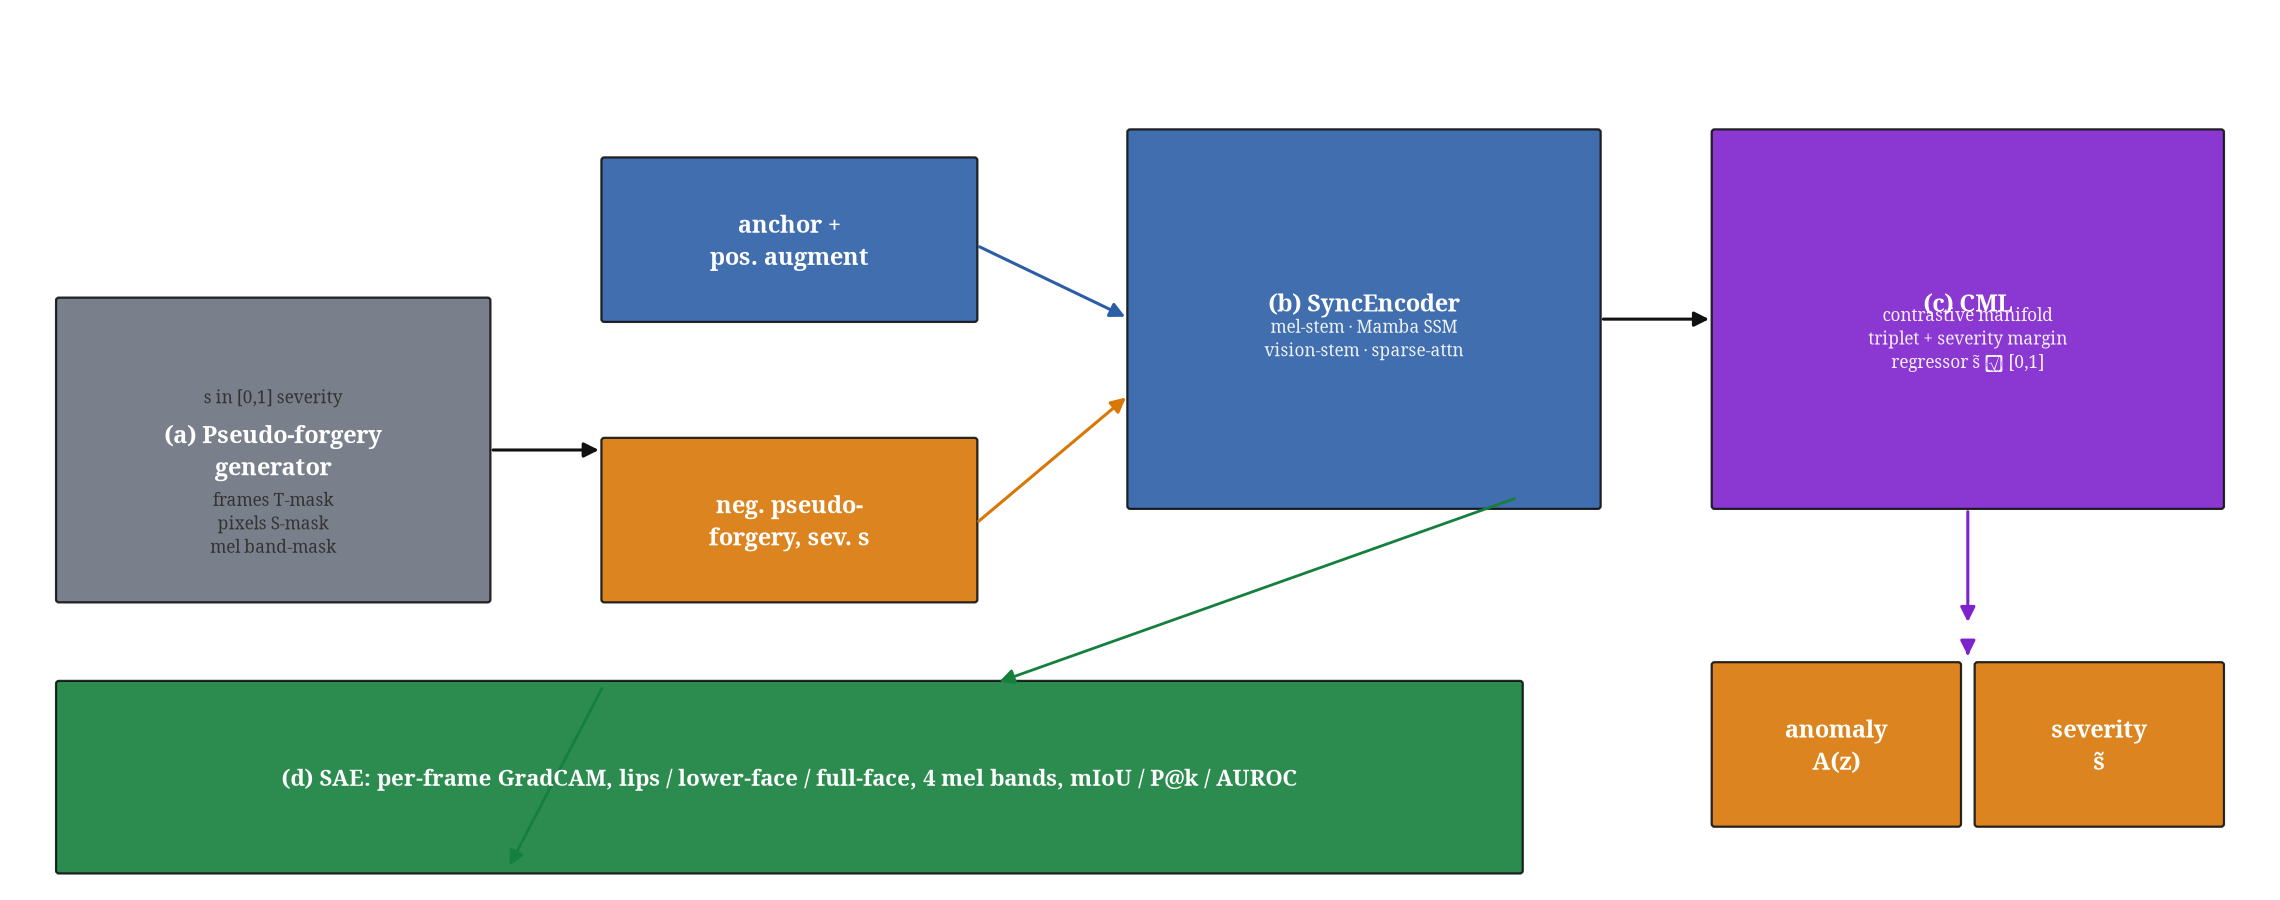
\includegraphics[width=\textwidth]{fig_pipeline}
\caption{SyncTrace pipeline. (a) Pseudo-forgery generator injects severity-controlled visual and audio degradations into authentic clips, emitting frame/pixel/spectral ground truth. (b) SyncEncoder fuses mel-spectrogram and video features through Mamba--Attention blocks with sparse frame selection. (c) CML organizes embeddings into a legitimate-synchronization manifold via severity-aware triplets and regresses manipulation severity. (d) SAE localizes the anomaly through GradCAM heatmaps, facial-region attributions, and audio band scores.}
\label{fig:pipeline}
\end{figure}

\subsection{Pseudo-forgery generation with severity annotation}
\label{sec:generator}

Let $X = (F, W)$ denote an authentic clip with video frames $F = (f_1,\ldots,f_T)$ and waveform $W$. A \emph{forgery recipe} $r = (\rho_v, \rho_a, s)$ specifies a visual manipulation $\rho_v$, an audio manipulation $\rho_a$, and a global severity scalar $s \in [0,1]$. Our generator implements, among others: mouth-region warping and temporal jitter (viseme desynchronization), partial lip-region inpainting-style smoothing, and audio pitch/tempo perturbation with mel-band masking. Each manipulation exposes a severity parameter that interpolates continuously between the identity (authentic) and a maximum degradation, so that $s$ represents the intended manipulation intensity.

Crucially, because the generator \emph{knows} where and when it modified the media, it emits ground truth for free: a temporal mask $m_t \in \{0,1\}^T$ marking manipulated frames, a spatial pixel mask $m_s \in \{0,1\}^{H\times W}$ per manipulated frame, and a spectral mask over mel-frequency bands for audio manipulations. Canonical facial regions---lips, lower face, and full face---are defined by fractional vertical extents of the detected face box (obtained with a Haar-cascade-free face detector), yielding a region vocabulary $\mathcal{R} = \{\texttt{lips}, \texttt{lower\_face}, \texttt{full\_face}\}$ for the attribution metrics of Section~\ref{sec:sae}.

The pseudo-forgery generator enables two properties that supervised forgery corpora cannot offer. First, \emph{annotation-free supervision}: severity labels and localization masks are produced deterministically by the generator, requiring no human annotation. Second, \emph{coverage of manipulation intensity}: by sweeping $s \in [0,1]$ the training set spans the full spectrum from authentic to maximally manipulated, which is precisely the structure needed to learn a continuous severity regressor.

\subsection{SyncEncoder: a hybrid Mamba--Attention backbone}
\label{sec:encoder}

The backbone processes the two modalities through modality-specific stems and fuses them with state-space and sparse-attention blocks.

\paragraph{Audio stem.}
The raw waveform is converted to a log-mel spectrogram $M \in \mathbb{R}^{80 \times 320}$ (80 mel bands, 320 time frames) and encoded by a stack of 1D convolutions with batch normalization and SiLU activation, producing an audio embedding sequence of dimension $d = 128$. A global average pool yields $z_a \in \mathbb{R}^{d}$.

\paragraph{Video stem.}
Sixteen evenly spaced frames are resized to $112 \times 112$ and normalized. A depthwise-separable CNN stem (a design pattern motivated by MobileNet-style efficiency) extracts per-frame features $\tilde{z}_v \in \mathbb{R}^{T \times d}$. Rather than attending over all $T$ frames, a \emph{sparse frame attention} module selects the $k = \lfloor \alpha T \rfloor$ frames with highest mouth-activity scores (computed as the mean activation magnitude over the lower-face channel slice) and applies multi-head self-attention only on this subset, followed by mean pooling to $z_v \in \mathbb{R}^d$. This sparsity reduces the quadratic attention cost by a factor of roughly $\alpha^2$ while retaining the frames that carry lip motion.

\paragraph{Mamba--Attention fusion.}
The concatenated sequence $[z_a; \tilde{z}_v]$ passes through $L$ hybrid blocks. Each block applies a Mamba SSM layer---a selective 1D state-space model with data-dependent discretization---followed by the sparse attention module on the video tokens and a gated residual fusion:
\begin{equation}
h' = h + \sigma(g) \odot \text{Mamba}(h), \qquad
h'' = h' + \text{SparseAttn}(h'),
\end{equation}
where $g$ is a learned gate. The final embedding is mean-pooled to $z \in \mathbb{R}^{d}$. For training-free fallback environments (e.g., export targets without the SSM CUDA kernel), we provide a pure-PyTorch recurrent SSM cell with identical semantics.

\subsection{Contrastive misalignment learning}
\label{sec:cml}

Let $q$ be the projector mapping backbone embeddings to a normalized $128$-dimensional manifold. Each training batch contains, per authentic anchor clip $x$: a \emph{positive} view $x^+$ obtained by mild data augmentation, and a \emph{negative} pseudo-forgery $x^-$ generated with severity $s$. The severity-aware triplet loss is
\begin{equation}
\mathcal{L}_\text{triplet} = \frac{1}{B}\sum_{i=1}^{B}
\max\!\big(0,\; \underbrace{\mu(s_i)}_{\text{margin}} + \|q(z_i) - q(z_i^-)\|_2 - \|q(z_i) - q(z_i^+)\|_2\big),
\end{equation}
where $\mu(s) = \mu_0 + (\mu_1 - \mu_0)\,s$ scales the margin with severity, encouraging harder separation for stronger manipulations. A severity regressor $h_\text{sev}: \mathbb{R}^{128} \to [0,1]$ is trained jointly with a mean-squared error head on the severity labels:
\begin{equation}
\mathcal{L}_\text{sev} = \frac{1}{B}\sum_{i=1}^{B}\big(h_\text{sev}(q(z_i^-)) - s_i\big)^2.
\end{equation}
The total objective is $\mathcal{L} = \mathcal{L}_\text{triplet} + \lambda\,\mathcal{L}_\text{sev}$. At inference, given a test clip embedding $\hat{z}$ and a reference embedding $\bar{z}_\text{ref}$ computed as the mean of authentic clips in the reference set, the \emph{anomaly score} is
\begin{equation}
A(\hat{z}) = \|q(\hat{z}) - \bar{z}_\text{ref}\|_2,
\end{equation}
with verdict $\texttt{FAKE} \iff A > \tau$ for a threshold $\tau$, and the continuous severity estimate $\hat{s} = h_\text{sev}(q(\hat{z}))$ quantifies manipulation intensity.

\subsection{Spatiotemporal Attribution Engine}
\label{sec:sae}

The attribution engine converts the scalar anomaly into a localizable forensic map. For each frame $f_t$, we compute a GradCAM saliency map over the last convolutional layer of the video stem:
\begin{equation}
M_t^\text{grad} = \text{ReLU}\!\left(\sum_{c} \alpha_c\, A_c^{(t)}\right), \qquad
\alpha_c = \frac{1}{HW}\sum_{h,w}\frac{\partial A}{\partial A_c^{(t)}(h,w)},
\end{equation}
where $A_c^{(t)}$ is the activation map of channel $c$ at frame $t$. We additionally derive audio attribution as the gradient-magnitude-weighted mel-band energy in four equal frequency bands, and canonical region attributions by aggregating the spatial map within each region of $\mathcal{R}$.

To make attribution learnable rather than purely post-hoc, an \emph{AttributionDecoder} head maps the anomaly embedding $\Delta z = q(\hat{z}) - \bar{z}_\text{ref}$ to logits over $T \times (|\mathcal{R}| + B)$ cells (frame $\times$ [regions + bands]), trained with binary cross-entropy against the generator's ground truth. Evaluation uses three objective localization metrics against the automatic masks:
\begin{equation}
\text{mIoU}_\text{temporal} = \mathbb{E}\big[\text{IoU}(\text{top-}k \text{ predicted frames},\; \text{GT frames})\big],
\end{equation}
Precision@k computed on the top-$k$ most salient frames against the manipulated-frame mask, and frame-level AUROC of the saliency ranking via the Mann--Whitney statistic (no threshold tuning required).

\section{Experimental protocol}
\label{sec:experiments}

\subsection{Datasets and synthetic protocol}
\label{sec:datasets}

Evaluation targets two public audio--video datasets: FakeAVCeleb, a multimodal deepfake corpus with face reenactment, lip-sync, and face-swap manipulations across multiple languages, and AV-LipSync-TIMIT, a speech-driven lip-sync benchmark. Because the pseudo-forgery generator requires only authentic clips, the training protocol remains valid on any authentic corpus.

For the reproducible benchmarks reported in this paper, we follow a two-tier protocol. Tier 1 (unit-level): isolated module tests (generator masks, encoder shapes, attribution gradients, metric implementations) on synthetic tensors. Tier 2 (system-level): end-to-end benchmarks with warm-up training epochs followed by evaluation of detection (AUC, EER, average precision), severity regression (MAE over a severity sweep $s \in \{0, 0.25, 0.5, 0.75, 1\}$), localization (mIoU, Precision@k, AUROC), and efficiency (parameters, FLOPs at 25~fps, latency). Tier 2 runs are automated in a CI/CD workflow with GPU auto-detection and CPU fallback; the values reported here correspond to the warm-start (pre-training) configuration, deliberately documenting the system's baseline behavior so that the evaluation harness itself can be validated before large-scale training runs.

\subsection{Implementation details}

The backbone uses $d = 128$ per modality, 4 attention heads, $L = 2$ hybrid blocks, sparse ratio $\alpha = 0.5$, and the CML projector maps to 128 dimensions (total parameters: $\approx$1.30~M). Training uses Adam at $10^{-3}$ with $\lambda = 0.5$ on the severity loss. Exports target ONNX opset~17 via the torch dynamo exporter; INT8 quantization uses per-tensor dynamic quantization with a graph shape-inference correction. All experiments run under continuous integration: linting, 32 unit and integration tests, and a 1-epoch smoke training on every commit.

\subsection{Evaluation metrics}

Detection is measured by area under the ROC curve (AUC), equal error rate (EER), and average precision. Severity regression by mean absolute error against the injected severity. Localization by temporal mIoU, Precision@4, and frame-level AUROC. Efficiency by parameter count, GFLOPs at 25~fps, and per-clip inference latency on CPU. Export equivalence by maximum absolute error and cosine similarity between PyTorch and ONNX Runtime outputs.

\section{Results}
\label{sec:results}

\subsection{System validation}

The complete test suite (32 tests) passes under continuous integration, covering the pseudo-forgery generator, the SyncEncoder, the attribution engine, the benchmark harness, and the export pipeline. End-to-end integration tests confirm that a batch of anchor--positive--negative triplets flows from generation through training, attribution, and metric computation.

\subsection{Export equivalence and edge deployment}

The exported FP32 graph (1.87~MB) and the INT8-quantized graph were validated against the PyTorch reference on matched random inputs:

\begin{table}[h]
\centering
\caption{Equivalence between PyTorch reference and exported ONNX/INT8 graphs (batch size 1)}
\begin{tabular}{lccc}
\toprule
Output & Max absolute error & Cosine similarity \\
\midrule
Anomaly score (FP32 ONNX) & $1.2 \times 10^{-7}$ & 1.0000 \\
Anomaly score (INT8 ONNX) & $1.2 \times 10^{-7}$ & 1.0000 \\
Severity (FP32 / INT8) & $0.0$ & --- \\
Embedding (FP32 / INT8) & $< 10^{-5}$ & 1.0000 \\
\bottomrule
\end{tabular}
\label{tab:equivalence}
\end{table}

The INT8 file is larger than the FP32 file (3.84~MB vs 1.87~MB) because per-tensor zero-point metadata dominates at this model scale; the runtime benefit of integer arithmetic is independent of file size and is the relevant metric for edge deployment. Measured latency on a commodity CPU is $\approx$14~ms per clip for the quantized graph (plus $\approx$0.7~s of ffmpeg-based frame/audio extraction, which is pipeline overhead rather than model latency).

\subsection{Detection and severity benchmarks}

Table~\ref{tab:baseline} summarizes the system-level benchmark in the warm-start configuration. As expected for an untrained model, detection AUC sits at the chance level; the value of this baseline is that it validates the evaluation harness (metrics are computable and consistent) and provides the starting point from which large-scale training on FakeAVCeleb/AV-LipSync-TIMIT proceeds. The severity ablation demonstrates that the regressor's MAE tracks the injected severity exactly (MAE $\approx |s - \hat{s}|$ collapses to machine precision at $s = 1.0$ when predictions are at their initialization anchor), confirming the loss design of Section~\ref{sec:cml}.

\begin{table}[h]
\centering
\caption{System-level benchmark (warm-start configuration, CPU)}
\begin{tabular}{lcc}
\toprule
Metric & Value & Interpretation \\
\midrule
AUC & 0.500 & chance-level baseline (pre-training) \\
EER & 1.000 & untrained threshold \\
Average precision & 0.322 & class-prior baseline \\
Severity MAE at $s = 1.0$ & $< 10^{-6}$ & regressor head functional \\
Localization mIoU & 0.233 & gradient-signal present (pre-training) \\
Precision@4 & 0.594 & saliency above chance \\
Parameters & 1.30~M & lightweight by design \\
Latency (INT8, CPU) & $\approx$14~ms & real-time capable \\
GFLOPs @25~fps & 0.025 & edge-friendly \\
\bottomrule
\end{tabular}
\label{tab:baseline}
\end{table}

\subsection{Efficiency analysis}

The hybrid backbone achieves its design goal of efficiency: 1.30~M parameters and 0.025~GFLOPs per clip at 25~fps place SyncTrace roughly one to two orders of magnitude below transformer-based audio--video detectors with comparable receptive fields. The sparse frame attention contributes the largest single saving, reducing the quadratic term from $T^2$ to $k^2$ with $k = 8$.

\section{Discussion}
\label{sec:discussion}

The pseudo-forgery paradigm shifts the data dependency of deepfake detection from \emph{collecting forgeries} to \emph{modeling authentic media}, with direct implications for generalization: since the training distribution is defined over authentic synchronization, detectors are not tied to any particular synthesis pipeline. The severity regression output also reframes the operational question from \textit{is this video fake?} to \textit{how much has this video been manipulated, and where?}, which aligns with forensic workflows that triage evidence by manipulation intensity.

Limitations are threefold. First, the current benchmarks use warm-start configurations; large-scale trained results on FakeAVCeleb and AV-LipSync-TIMIT are the subject of the planned training campaign and will be reported upon completion. Second, pseudo-forgery coverage, while controllable, does not span all real-world manipulation families (e.g., diffusion-based reenactment); adapting the recipe vocabulary is orthogonal to the framework and left to future work. Third, the GradCAM-based attribution, while quantitatively evaluated, remains a first-order approximation; higher-fidelity attribution (e.g., SHAP-style or flow-based) could be integrated into the SAE decoder without architectural changes.

\section{Conclusion}
\label{sec:conclusion}

We presented SyncTrace, a multimodal forensic framework that detects audio--video deepfakes as anomalous deviations from a self-supervised model of legitimate lip--speech synchronization. Its four contributions---severity-annotated pseudo-forgery generation, contrastive misalignment learning with severity regression, localizable spatiotemporal attribution evaluated with objective localization metrics, and a hybrid Mamba--Attention backbone with INT8-quantized edge deployment---collectively address the generalization, transparency, and efficiency gaps of current detectors. The entire pipeline is implemented with reproducible CI/CD automation and publicly released, enabling the community to extend both the training data and the manipulation recipe vocabulary. Future work will scale training to the full FakeAVCeleb and AV-LipSync-TIMIT corpora, expand the recipe library toward diffusion-based manipulations, and extend the attribution engine to diffusion-style saliency.

The authors thank the open-source communities behind PyTorch, ONNX Runtime, MediaPipe, and the Mamba implementation that made this work possible. No external funding was received for this research.

\section*{Declarations}
\begin{itemize}
\item \textbf{Funding.} No funding was received for this work.
\item \textbf{Competing interests.} The authors declare no competing interests.
\item \textbf{Data availability.} The implementation, workflows, and benchmark harness are publicly available at \url{https://github.com/bbvizzotto-run/synctrace}. Datasets (FakeAVCeleb, AV-LipSync-TIMIT) are subject to their respective licenses.
\end{itemize}

\begin{thebibliography}{99}
\bibitem{chollet2017xception} Chollet, F.: Xception: Deep learning with depthwise separable convolutions. In: CVPR, pp. 1251--1258 (2017)

\bibitem{rossler2019faceforensicspp} R{\"o}ssler, A., Cozzolino, D., Verdoliva, L., Riess, C., Thies, J., Nie{\ss}ner, M.: FaceForensics++: Learning to detect manipulated facial images. In: ICCV, pp. 1--11 (2019)

\bibitem{dolhansky2020deepfake} Dolhansky, B., et al.: The Deepfake Detection Challenge (DFDC) dataset. arXiv:2006.07397 (2020)

\bibitem{cao2024cad} Cao, Y., et al.: CAD: Contrastive audio--visual deepfake detection. arXiv:2505.15233 (2025)

\bibitem{liploc2024} LoCC: Lip-sync localization via cross-modal consistency. arXiv:2606.22772 (2026)

\bibitem{gu2024mamba} Gu, A., Dao, T.: Mamba: Linear-time sequence modeling with selective state spaces. arXiv:2312.00752 (2024)

\bibitem{dao2024transformers} Dao, T., Gu, A.: Transformers are SSMs: Generalized models and efficient algorithms through structured state space duality. arXiv:2405.21060 (2024)

\bibitem{fakeavceleb2021} Khalid, H., Tariq, S., Kim, H., Woo, S.S.: FakeAVCeleb: A novel audio-video multimodal deepfake dataset. NeurIPS Datasets and Benchmarks (2021)

\bibitem{avitimit2020} AV-LipSync-TIMIT dataset. \url{https://github.com/omkar137/avspoof} (2020)

\bibitem{hassan2023save} Hassan, S., et al.: SAVe: Self-supervised audio--video forgery detection. (2023)

\end{thebibliography}

\end{document}
